%!TeX spellcheck = ru_GB
\documentclass[12pt,a4paper]{article}
\usepackage[warn]{mathtext}
\usepackage[T2A]{fontenc}
\usepackage[utf8x]{inputenc}
\usepackage{ucs}
\usepackage{adjustbox}
\usepackage{upgreek}
\usepackage[english, russian]{babel}
\usepackage{graphicx}

\usepackage{textcomp}
\usepackage{cmap}
\usepackage[OT1]{fontenc}
\usepackage{mathtools}
\usepackage{amsfonts}
\usepackage{amssymb}
\usepackage{enumitem}
\usepackage{alltt}
\setcounter{secnumdepth}{0}
\usepackage{indentfirst}
\usepackage{caption}
\usepackage{float}
\usepackage{wrapfig}
\usepackage{physics}
\usepackage{multirow}
\usepackage{longtable}
\captionsetup{justification=centering}
\RequirePackage[singlelinecheck=off]{caption}
\usepackage{amsmath,amsfonts,amssymb,amsthm,mathtools}
\usepackage{icomma}
\setlength{\parindent}{0.75cm}
\graphicspath{{pictures/}}
\DeclareGraphicsExtensions{.png, .jpg}
\usepackage{subcaption}
\DeclareCaptionFormat{subfig}{\figurename~#1#2#3}
\DeclareCaptionSubType*{figure}
\captionsetup[subfigure]{format=subfig,labelsep=colon, labelformat=simple}
\usepackage{wrapfig}
\usepackage[left=15mm,right=15mm,top=2cm,bottom=2cm]{geometry}
\author{Кравец Кирилл}

\begin{document}
	
	\begin{titlepage}
		\centering
		\vspace{5cm}
		{\scshape\LARGE Московский физико-технический институт \par}
		\vspace{4cm}
		{\scshape\Large Лабораторная работа 1. \par}
		\vspace{1cm}
		{\huge\bfseries Измерение температуры пламени методом обращения спектральных линий. \par}
		\vspace{1cm}
		\vfill
		\begin{flushright}
			{\large выполнили: }\par
			\vspace{0.3cm}
			{\LARGE 
			Рогозин Владимир\\
			Герасимов Илья\\
			Кравец Кирилл\\
			Казусев Степан\\
			Дюгаева Юлия}
		\end{flushright}
		
		
		\vfill
		
		% Bottom of the page
		Долгопрудный, 2023 г.
	\end{titlepage}
	
	\textbf{Цель работы}: изучение процессов теплообмена между пламенем пропановой горелки и металлической пластины, внесённой в пламя.\\
	
	
	\textbf{В работе используются}: пирометр ЛОП-72, горелка, горючее, компрессор, фитилёк, смоченный раствором поваренной соли, фотометрическая лампа.\\
	
	\textbf{Методика измерения}:\\ 
	В данной лабораторной работе измерения температуры проводятся двумя способами:\\
	а) пирометрическим, с помощью которого измеряется температура раскалённых металлов,\\
	б) методом обращения спектральных линий, с помощью которого определяется температура пламени пропановой горелки.
	
	\section*{Теоретические сведения}
	
	Введём понятие спектральной интенсивности излучения $I_\lambda dS dt d\lambda d\Omega$ - количество энергии, переносимой излучением через площадку единичной площади, нормаль которой совпадает с направлением распространения излучения, за единицу времени, в единичном спектральном интервале длин волн, в единичном телесном угле.
	
	\begin{figure}[H]
		\centering
		\includegraphics[scale=1]{"C:/working folder/mss_labs_RGKKD/1"}
		\caption{К понятию интенсивности излучения}
		\label{fig:1}
	\end{figure}

	В случае изотропного (диффузного) излучения с поверхности dS энергия, излучаемая за время dt внутри телесного угла d$\Omega$ в интервале волн $d\lambda$ равна:
	
	\begin{equation}
		dU = E_\lambda(T)cos(\phi)d\lambda dS d\Omega dt - \text{закон Ламберта}
	\end{equation}
	
	Для вычисления полного количества энергии, излучаемой элементом диффузной поверхности используют соотношение: 
	
	\begin{equation}
		\frac{dU}{dt} = K_\lambda(T)dSd\lambda = \pi E_\lambda(T)dS d\lambda,
	\end{equation}

	Где $ K_\lambda(T)$ иногда называют полусферической спектральной поверхностной плотностью излучения. Соотношение (2) показывает, что полная испускаемая энергия, изпускаемая элементов поверхности dS, в $\pi$ раз больше энергии, излучаемой им в направлении нормали к поверхности в пределах единичного телесного угла.\\
	
	Рассмотрим падение излучения  $I_\lambda^0$ на произвольное тело.
	
	Часть этого излучения может поглотиться телом $I_\lambda^A$, часть - отразиться $I_\lambda^R$, а часть - пройти сквозь тело без изменения $I_\lambda^D$.
	
	Из закона сохранения энергии:
	\begin{equation}
		I_\lambda^0 = I_\lambda^R + I_\lambda^A + I_\lambda^D.
	\end{equation}


	\begin{figure}[H]
		\centering
		\includegraphics[scale=1]{"C:/working folder/mss_labs_RGKKD/2"}
		\caption{Различные процессы, связанные с излучением.}
		\label{fig:2}
	\end{figure}

	Введём следующие понятия:
	
	\begin{equation}
		R_\lambda = \frac{I_\lambda^R}{I_\lambda^0}  - \text{спектральная отражательная способность} 
	\end{equation}
	
	\begin{equation}
		A_\lambda = \frac{I_\lambda^A}{I_\lambda^0}  - \text{спектральная поглощательная способность} 
	\end{equation}
	
	\begin{equation}
		D_\lambda = \frac{I_\lambda^D}{I_\lambda^0}  - \text{спектральная пропускательная способность} 
	\end{equation}
	
	\begin{equation}
		R_\lambda + A_\lambda + D_\lambda = 1.
	\end{equation}
	
	Тело, которое полностью поглощает падающее на него излучение произвольной частоты, называется абсолютно чёрным телом. Для него $A_\lambda$ = 1. Для любого вещества отношение лучеиспускательной способности к поглощательной одинаково для всех  веществ и равно спектральной интенсивности чёрного излучения $B_\lambda(T)$.
	
	\begin{equation}
		\frac{E_\lambda(T)}{A_\lambda} = B_\lambda(T)  -  \text{закон Кирхгофа}.
	\end{equation}

	Для абсолютно чёрного тела интенсивность излучения равна интенсивности теплового равновесного излучения при одинаковой температуре.
	
	\begin{equation}
		E_\lambda(T)= B_\lambda(T) 
	\end{equation}

	Функция $B_\lambda$(T) одинакова для всех веществ:
	
	\begin{equation}
		B_\lambda(T) = \frac{2hc^2}{\lambda^5(e^{\frac{hc}{\lambda kT}} - 1)} - \text{закон распределения Планка}
	\end{equation}

	c - скорость света в вакууме, h - постоянная Планка, k  -  постоянная Больцмана. 
	
\begin{figure}[H]
	\centering
	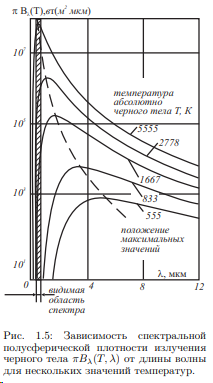
\includegraphics[scale=1.2]{3}
	\caption{}
	\label{fig:3}
\end{figure}

	Из закона распределения Планка следует закон Стефана-Больцмана:
	
\begin{equation}
	N_s(T) = \sigma_s T^4, \; где \; \sigma_S = 5.67 \cdot 10^{-8} Вт/м^2 \cdot К^4
\end{equation}

Введём величину $\varepsilon_{\lambda}(T)$, называемую степенью черноты тела:

\begin{equation}
	\varepsilon_{\lambda}(T) = \frac{U_s \; \text{(истинная)}}{U_s \; \text{(Стефан-Больцман)}} = 
	\frac{E_\lambda(T)}{B_\lambda(T)}
\end{equation}

где U обозначает физическую величину энергии, проходящей через площадку за единицу времени.

В данной лабораторной работе будет рассматриваться  степень черноты в направлении нормали, которая по закону Кирхгофа совпадает с определением поглощательной способности: 

\begin{equation}
	\varepsilon_{\lambda, n}(T) = A_\lambda(T).
\end{equation}  


	
	\section{Экспериментальная установка}
	
	Пирометры - приборы, используемые для исследования излучения раскалённого объекта.
	Работа пирометра основана на сравнении интенсивности света, излучаемого, с одной стороны, объектом и, с другой стороны, фотометрической лампой накаливания.\\
	
	\textbf{Принцип измерения с исчезающей нитью}\\
	Принцип устройства пирометра с исчезающей нитью представлен на рисунке 4.
	
	\begin{figure}[H]
		\centering
		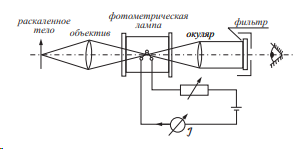
\includegraphics[scale=1.5]{4}
		\caption{}
		\label{fig:4}
	\end{figure}

	Фильтр пропускает свет с длиной волны $\lambda$ в интервале длин волн $\Delta$$\lambda$. Изображение части светящейся поверхности тела и нити лампы наблюдается одновременно с помощью окуляра. Значение тока J, соответствующее равенству интенсивностей излучения нити и изображения, позволяет измерить температуру тела с использованием предварительной калибровки прибора по черному телу.
	
	Параметры градуируются по излучению чёрного тела. 
	
	Далее можно получить соотношение для истинной температуры тела.
	
	\begin{equation}
		\frac{1}{T} = \frac{1}{T_b} + \frac{\lambda}{C_2} ln\overline{\varepsilon}_{\lambda, n}
	\end{equation}\\

	Где $T_b$ - яркостная температура (температура излучаемого тела = температуре абс. чёрного тела с тем же тепловым излучением). $\overline{\varepsilon}_{\lambda, n}$ - среднее значение cтепени черноты нагретого тела, меньше единицы. 
	
	
	
	
	\textbf{Принцип измерения методом обращения спектральных линий}\\
	Схема измерения температуры пламени методом обращения спектральных линий приведена на рис.5.
	
	\begin{figure}[H]
		\centering
		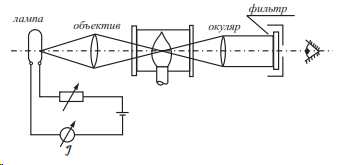
\includegraphics[scale=1.2]{5}
		\caption{}
		\label{fig:5}
	\end{figure}
	
	\begin{figure}[H]
		\centering
		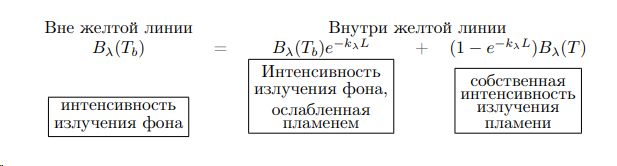
\includegraphics[scale=1]{6}
		\caption{}
		\label{fig:6}
	\end{figure}
	
	$T_b$ - яркостная температура лампы, T - температура пламени, $k_\lambda$ - спектральный коэффициент поглощения пламени при температуре T, L - толщина излучающего слоя пламени.
	
	Из (6) следует: $B_\lambda(T_b) = B_\lambda(T)$, $T_b = T$.
	
	То есть если осуществляется баланс интенсивностей, то температура пламени равна яркостной температуре фотометрической лампы.
	
	В реальных измерительных системах фильтр заменяется монохроматором. Излучение пламени и лампы просвечивания фокусируется на входную щель монохроматора, и после прохождения через диспергирующий элемент внутри монохроматора на выходе наблюдают спектр. Увеличивая ток через лампу можно наблюдать, что яркие вначале по отношению к фону линии затем наоборот станут темнее фона. От этого и идёт название метода - мeтод обращения спектральных линий.

	
	
	\section*{Ход работы}
	
	\noindent 1. Соберём схему для измерения температуры пламени методом обращения спектральных линий. \\
	
	\noindent 2. Зажжём горелку. Регулируя подачу горючего добьёмся устойчивого пламени. Регулируя поступление воздуха, добьёмся устойчивого пламени. Внесём в пламя фитилёк, смоченный раствором поваренной соли.\\
	
	\noindent 3. Добъёмся чёткой видимости свечения резонансных линий натрия в окуляре монохроматора ($\lambda_{N_a}$ = 0.5890; 0.5896 мкм).\\
	
	\noindent 4. Изменяя величину электрического тока через фотометрическую лампу, добъёмся исчезновения линий натрия на фоне изображения ленты фотометрической лампы.\\
	
	\noindent 5. С помощью пирометра определим яркостную температуру лампы. В таблице приведены значения тока I, соответствующего равенству интенсивностей излучения нити и изображения для различных наблюдателей. I' - ток лампы пирометра.
	
	\begin{table}[H]
		\centering
		\begin{tabular}{|c|c|c|}
			\hline
			№ & I, A                      & I', A \\ \hline
			1 & 17.6                      & 0.345 \\ \hline
			2 & 17.6                      & 0.345 \\ \hline
			3 & 17.8                      & 0.345 \\ \hline
			4 & 18.1					  & 0.35  \\ \hline
			5 & 18.0					  &  -	  \\ \hline
		\end{tabular}
	\end{table}
	
	Среднее значение I выборки из 5-ти опытов соответствует:
	
	\begin{equation}
		I =  17.82 \pm 0.2 A. \; I' = 0.345 \pm 0.04 A;
	\end{equation}

	Следовательно $T_b$ = (1900 $\pm$ 25) K. (участок II на графике (7),т.к. использовали фильтр-поглотитель)

\begin{figure}[H]
	\centering
	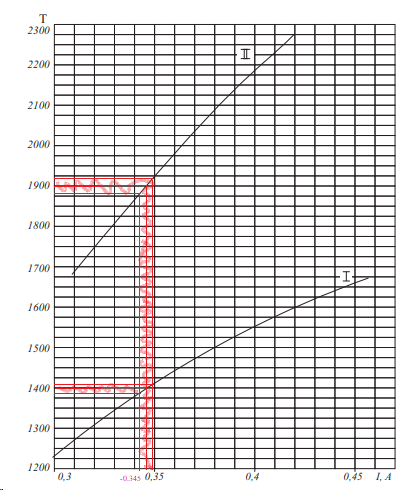
\includegraphics[scale=1.2]{7}
	\caption{Калибровочные кривые для определения яркостной температуры}
	\label{fig:7}
\end{figure}
	
	
	Найдём значение степени черноты в направлении нормали для исследуемой вольфрамовой нити по  графику зависимости полусферической степени черноты вольфрама $\varepsilon_{\lambda}(T)$ от длины волны $\lambda$ и температуры поверхности T K. 	За длину волны излучения вольфрамовой нити приняли $\lambda$ = 0.5890 мкм.
	
	\begin{figure}[H]
		\centering
		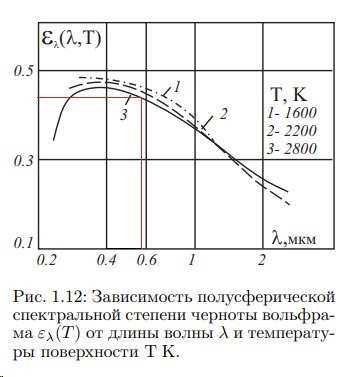
\includegraphics[scale=1.2]{8}
		\caption{}
		\label{fig:8}
	\end{figure}

	
	\begin{equation}
		\varepsilon_{\lambda, n} = 0.44 \pm 0.3
	\end{equation}

	Найдем истинную температуру пламени: 

	\begin{equation}
		T = \frac{1}{\frac{1}{T_b} + \frac{\lambda}{0.0144}\ln(0.44)} = 2029 \pm 30 \; K.
	\end{equation}
	
	\section{Выводы}
	
	В монохроматоре был получен различимый дуплет линий спектра жёлтого дуплета натрия. С помощью значений тока на пирометре и тарировочной кривой были получены яркостная температура лампы накаливания (1900 $\pm$ 25 К) и истинная температура пламени (2029 $\pm$ 30 К). По
	теории сходится то, что истинная температура должна быть выше, чем яркостная температура.
	
	
\end{document}